%%
%% CoopIDS — Graduate Research Project Report
%% ACM Master Article Template (sigconf)
%%
\documentclass[sigconf,nonacm]{acmart}

\usepackage{booktabs}
\usepackage{multirow}
\usepackage{amsmath}
\usepackage{algorithm}
\usepackage{algpseudocode}
\usepackage{graphicx}
\usepackage{xcolor}
\usepackage{subcaption}

\setcopyright{none}
\copyrightyear{2026}
\acmYear{2026}
\acmDOI{XXXXXXX.XXXXXXX}
\acmConference[]{ECE752}{April 2, 2026}{Waterloo, ON}
\pagestyle{plain}

\begin{document}

\title{CoopIDS: Cooperative Multi-Agent Reinforcement Learning\\for DDoS Mitigation at ISP Edge Routers}

\author{Abdenour Belarbi}
\affiliation{%
  \institution{University of Waterloo}
  \city{Waterloo}
  \state{Ontario}
  \country{Canada}
}
\email{abdenour.belarbi@uwaterloo.ca}

\renewcommand{\shortauthors}{Belarbi}

\begin{abstract}
Distributed Denial-of-Service (DDoS) attacks remain a critical threat to cloud infrastructure, while existing defenses often rely on single-point detection or coarse traffic filtering that fails against coordinated, multi-vector attacks. We propose \textbf{CoopIDS}, a cooperative multi-agent reinforcement learning framework for intelligent DDoS mitigation at ISP edge routers. CoopIDS agents learn fine-grained, per-flow filtering policies and coordinate across distributed routers via centralized training with decentralized execution. We evaluate CoopIDS on real-world cloud traffic covering both seen and unseen attack types, achieving 99.5\% detection on known attacks and strong generalisation to unseen attacks (up to 93.83\% F1 score). A 40-stage ablation study shows that while the learned policies generalise effectively, performance is primarily limited by the risk-scoring component, identifying it as the key bottleneck and a clear direction for future improvement.
\end{abstract}

\begin{CCSXML}
<ccs2012>
  <concept>
    <concept_id>10010147.10010178.10010187</concept_id>
    <concept_desc>Computing methodologies~Multi-agent systems</concept_desc>
    <concept_significance>500</concept_significance>
  </concept>
  <concept>
    <concept_id>10010147.10010178.10010179</concept_id>
    <concept_desc>Computing methodologies~Reinforcement learning</concept_desc>
    <concept_significance>500</concept_significance>
  </concept>
  <concept>
    <concept_id>10002978.10002986.10002990</concept_id>
    <concept_desc>Security and privacy~Intrusion detection systems</concept_desc>
    <concept_significance>300</concept_significance>
  </concept>
  <concept>
    <concept_id>10003033.10003068.10003073</concept_id>
    <concept_desc>Networks~Network security</concept_desc>
    <concept_significance>300</concept_significance>
  </concept>
</ccs2012>
\end{CCSXML}

\ccsdesc[500]{Computing methodologies~Multi-agent systems}
\ccsdesc[500]{Computing methodologies~Reinforcement learning}
\ccsdesc[300]{Security and privacy~Intrusion detection systems}
\ccsdesc[300]{Networks~Network security}

\keywords{Multi-Agent Reinforcement Learning, DDoS Mitigation, Cooperative IDS, MAPPO, CTDE, Network Security}

\maketitle

%% ═══════════════════════════════════════════════════════════════════
\section{Introduction}
\label{sec:intro}

Distributed Denial-of-Service (DDoS) attacks have grown in both sophistication and volume, with modern TCP-based floods designed to evade signature-based detection by mimicking legitimate connection patterns~\cite{mirkovic2004taxonomy}. Traditional Intrusion Detection Systems (IDS) such as Snort and Suricata operate as centralised, single-point classifiers: they observe traffic from one vantage point, apply static rules, and make binary block-or-forward decisions. This architecture suffers from three fundamental limitations: (1) a single sensor cannot observe the full spatial distribution of a multi-vector attack, (2) binary actions cannot express graduated confidence---a flow that is 60\% suspicious warrants different treatment than one that is 95\% malicious, and (3) static rules fail to generalise to novel attack patterns.

Multi-Agent Reinforcement Learning (MARL) offers a compelling alternative: multiple learning agents deployed at distributed network nodes can observe local traffic patterns, share information through centralised training, and adapt their responses in real time. However, prior MARL-based approaches to DDoS mitigation~\cite{malialis2015distributed} have used synthetic traffic, volumetric-only attacks, and blind throttling actions that drop all traffic equally regardless of flow-level risk.

We present \textbf{CoopIDS} (Cooperative Intrusion Detection System), a MARL framework that addresses these limitations through three key innovations:

\begin{enumerate}
    \item \textbf{Per-flow risk-driven routing:} A pre-trained LightGBM 3-class classifier assigns each flow a risk score $p_\text{risk} = 1 - P(\text{benign})$, which determines how the flow is routed through the selected tiered action profile.

    \item \textbf{Tiered action profiles:} Instead of binary block/forward or explicit throttle rates, agents select from six predefined profiles (passive $\to$ lockdown), each specifying thresholds $(T_\text{block}, T_\text{puzzle})$ that determine per-flow treatment.

    \item \textbf{Cooperative CTDE architecture:} Using Multi-Agent PPO (MAPPO) with a centralised critic that observes all agents' states during training, agents learn to coordinate their filtering strategies while executing independently at deployment time.
\end{enumerate}

We evaluate CoopIDS on the BCCC-cPacket-Cloud-DDoS-2024 dataset~\cite{bccc2024}, which contains real cloud traffic captured from AWS infrastructure including 12 TCP-based attack types on Monday and 5 completely different attack types on Tuesday. This setup enables rigorous zero-shot generalisation testing: the policy is trained exclusively on Monday data and evaluated on Tuesday without any retraining.

Our research addresses three questions:
\begin{itemize}
    \item[\textbf{RQ1}] Can cooperative MARL at ISP routers stop real DDoS flows intelligently, without indiscriminate traffic dropping?
    \item[\textbf{RQ2}] Does the learned policy generalise zero-shot to attack types never seen during training?
    \item[\textbf{RQ3}] What limits generalisation---the RL policy or the risk sensor?
\end{itemize}

Through a systematic 40-stage ablation study (S1--S40), we demonstrate that CoopIDS generalises zero-shot to unseen attacks with up to 93.83\% F1, and that the primary bottleneck for generalisation is the risk sensor rather than the learned policy.


%% ═══════════════════════════════════════════════════════════════════
\section{Related Work}
\label{sec:related}

\subsection{Traditional DDoS Detection}

Signature-based IDS (Snort~\cite{roesch1999snort}, Suricata) detect known attack patterns through predefined rules but fundamentally cannot generalise to unseen variants. These systems have been the industry standard for decades, offering low latency and high throughput, but their rule databases require manual curation and fail to detect zero-day attacks or novel evasion techniques.

Machine-learning approaches have progressively replaced or augmented signature-based systems. Random Forests~\cite{breiman2001random} and gradient-boosted trees~\cite{ke2017lightgbm} achieve high accuracy on structured flow-level features, while deep learning approaches (autoencoders, CNNs, LSTMs) have been applied to raw packet data or time-series traffic analysis~\cite{mirsky2018kitsune}. However, all these approaches operate as single-point classifiers: they observe traffic from one vantage point and make independent predictions. In a distributed attack where malicious flows arrive through multiple ingress points, no single classifier has a complete view of the attack topology.

\subsection{MARL for Network Security}

Malialis et al.~\cite{malialis2015distributed} pioneered the use of multi-agent RL for DDoS response, deploying tabular Q-learning agents at distributed network nodes. Their agents learn to throttle traffic rates when under attack, reducing the volume of forwarded flows. While groundbreaking, their approach has several limitations: (1) agents use synthetic traffic generators rather than real attack traces, (2) only volumetric (bandwidth-exhaustion) attacks are considered---modern TCP floods that mimic legitimate connections would evade their detectors, (3) the throttling action is \emph{blind}, dropping all traffic at a chosen rate regardless of individual flow risk, and (4) agents train independently without cooperation mechanisms, preventing coordinated response.

Subsequent surveys~\cite{han2021marl} have identified the potential for MARL in broader network defence scenarios, including intrusion detection, autonomous penetration testing, and network configuration optimisation. However, to our knowledge, no prior work has demonstrated MARL-based per-flow DDoS mitigation on real cloud traffic with zero-shot generalisation to unseen attack types.

\subsection{Cooperative Multi-Agent RL}

The Centralized Training with Decentralized Execution (CTDE) paradigm~\cite{lowe2017multi} addresses the fundamental challenge of multi-agent credit assignment: during training, a centralised component (critic, mixing network, or communication channel) enables agents to reason about joint actions, while at deployment time, agents act independently using only local observations. This paradigm is particularly relevant for network security, where a centralised training server can aggregate telemetry from all routers, but execution must be decentralized due to latency constraints.

Multi-Agent PPO (MAPPO)~\cite{yu2022surprising} extends Proximal Policy Optimization~\cite{schulman2017proximal} to multi-agent settings with a shared centralised critic. Yu et al. demonstrated that MAPPO, despite its simplicity, achieves surprisingly strong performance across cooperative benchmarks including StarCraft Multi-Agent Challenge and Google Research Football. The key insight is that parameter sharing between agents, combined with a centralised value function, provides sufficient coordination for many cooperative tasks.

Independent PPO (IPPO), where each agent trains with only its own local critic, provides a natural ablation baseline. IPPO has been shown to match MAPPO in some cooperative settings~\cite{de2020independent}, raising the question of when centralised critics provide meaningful benefit---a question our scaling experiments (3 vs 6 routers) directly address.

\subsection{Risk-Based Network Filtering}

Puzzle-based defences such as CAPTCHA challenges and proof-of-work (PoW) requirements~\cite{wang2003detecting} provide an intermediate action between blocking and forwarding. By requiring computational effort to pass, puzzles impose asymmetric costs: legitimate users (with real browsers or clients) can solve challenges, while botnets cannot cost-effectively solve them at scale. Our tiered profile approach extends this concept by coupling puzzle thresholds with blocking thresholds into coherent defensive postures, creating a graduated response spectrum that maps naturally to the agent's discrete action space.


%% ═══════════════════════════════════════════════════════════════════
\section{Methodology}
\label{sec:method}

CoopIDS consists of three integrated components: a per-flow risk scorer, a multi-agent environment with tiered action profiles, and the MAPPO training algorithm.

\subsection{Dataset: BCCC-cPacket-Cloud-DDoS-2024}

We use the BCCC-cPacket-Cloud-DDoS-2024 dataset~\cite{bccc2024}, which captures real DDoS traffic from AWS cloud infrastructure. The dataset spans multiple days, with each day containing different attack campaigns:

\begin{itemize}
    \item \textbf{Monday} (320,530 flows): 12 TCP attack types (68.7\% attack, 21.4\% benign, 9.9\% suspicious), targeting 6 victim machines through 20-minute attack blocks across an 8-hour window.
    \item \textbf{Tuesday} (85,479 flows): 5 completely unseen attack types (TCP-Flag-RST-ACK, TCP-Flag-SYN-TFO, TCP-Flag-SYN-TIME, TCP-Flag-OSYN, TCP-Flag-OSYNP).
\end{itemize}

The monday--Tuesday split provides natural zero-shot evaluation: no Tuesday attack type appears in Monday's training data, while the underlying benign traffic distributions differ across days.

\subsection{Per-Flow Risk Scoring}
\label{sec:risk}

We employ a LightGBM~\cite{ke2017lightgbm} gradient-boosted classifier trained on Monday data with 42 selected flow-level features to produce three class probabilities per flow: $P(\text{attack})$, $P(\text{benign})$, and $P(\text{suspicious})$.

From these probabilities, we derive a single risk score:
\begin{equation}
    p_\text{risk} = 1 - P(\text{benign})
    \label{eq:prisk}
\end{equation}

This formulation is critical for generalisation. On unseen Tuesday attacks, the classifier's $P(\text{attack})$ degrades significantly (mean gap between attack and benign windows drops from 0.765 to 0.268). However, $p_\text{risk} = 1 - P(\text{benign})$ remains discriminative because the model can still identify when traffic is \emph{not} benign, even when it cannot distinguish between attack and suspicious categories.

\subsection{Multi-Agent Environment}
\label{sec:env}

\subsubsection{Network Topology}

We simulate $N = 3$ ISP edge routers, each responsible for a subset of source IPs assigned via consistent hashing:
\begin{equation}
    \text{agent}(f) = \text{hash}(\text{src\_ip}(f)) \bmod N
    \label{eq:routing_assign}
\end{equation}
This ensures all flows from the same source IP are always handled by the same router, preserving per-source temporal context. Each router processes its flows independently but the agents coordinate through CTDE during training.

\subsubsection{Time Windows}

Traffic is segmented into 30-second windows. Within each window, the router collects all flows assigned to it, computes aggregate statistics, and selects an action that determines the filtering policy for the next window. A full Monday episode spans approximately 968 windows (08:56--17:00).

\subsubsection{State Representation}

Each agent observes a 4-dimensional local state at each time step:
\begin{equation}
    s_i^t = \left[\bar{p}_\text{atk},\; \bar{p}_\text{ben},\; \bar{p}_\text{sus},\; \frac{n_\text{flows}}{\text{MAX\_FLOWS}}\right]
    \label{eq:state}
\end{equation}
where $\bar{p}_\text{atk}$, $\bar{p}_\text{ben}$, $\bar{p}_\text{sus}$ are the mean class probabilities across all flows in the window, and $n_\text{flows}$ is normalised by a maximum of 1{,}000 flows.

\subsubsection{Tiered Action Profiles}
\label{sec:tiers}

Each agent selects from 6 tiered action profiles $a \in \{0, \ldots, 5\}$, each specifying two per-flow routing thresholds $(T_\text{block}, T_\text{puzzle})$ calibrated from the Monday $p_\text{risk}$ distribution, spanning from no blocking (Passive, $T_\text{block}=1.00$) to maximum blocking (Lockdown, $T_\text{block}=0.50$):

\begin{table}[h]
\centering
\small
\caption{Tiered action profiles. Thresholds calibrated from Monday $p_\text{risk}$ distributions: $T_\text{block}$ spaced uniformly over the discriminative range $[0.50, 1.00]$; $T_\text{puzzle}$ set to capture the ambiguous band below each blocking threshold.}
\label{tab:profiles}
\begin{tabular}{clccc}
\toprule
Action & Profile & $T_\text{block}$ & $T_\text{puzzle}$ & Puzzle band width \\
\midrule
0 & Passive    & 1.00 & 1.00 & --- \\
1 & Light      & 0.90 & 0.60 & 0.30 \\
2 & Moderate   & 0.80 & 0.40 & 0.40 \\
3 & Firm       & 0.70 & 0.25 & 0.45 \\
4 & Aggressive & 0.60 & 0.15 & 0.45 \\
5 & Lockdown   & 0.50 & 0.10 & 0.40 \\
\bottomrule
\end{tabular}
\end{table}

For each flow $f$, the routing decision under the selected profile is:
\begin{equation}
    \text{decision}(f) = \begin{cases}
        \text{BLOCK}   & \text{if } p_\text{risk}(f) \geq T_\text{block} \\
        \text{PUZZLE}  & \text{if } p_\text{risk}(f) \geq T_\text{puzzle} \\
        \text{FORWARD} & \text{otherwise}
    \end{cases}
    \label{eq:routing}
\end{equation}

Flows routed to PUZZLE undergo a computational challenge with pass rates: benign flows pass with probability 0.95, suspicious flows with 0.50, and attack flows with 0.05, modelling realistic CAPTCHA/PoW systems. The agent's action selection thus controls \emph{how aggressively} the $p_\text{risk}$ signal is exploited on a per-window basis, while the flow-level routing within that window is handled deterministically by the thresholds.

\subsubsection{Reward Function}

We use a local reward per agent $i$:
\begin{equation}
    r_i^t = \frac{n_\text{benign\_passed}^i}{n_\text{benign\_total}^i} - \frac{n_\text{attack\_passed}^i}{n_\text{attack\_total}^i}
    \label{eq:reward}
\end{equation}

This balances two objectives: preserving legitimate traffic (first term) while blocking attacks (second term). The reward lies in $[-1, 1]$, with $r = 1$ representing perfect filtering (all benign forwarded, all attacks blocked).

\subsection{MAPPO with CTDE}
\label{sec:mappo}

We use Multi-Agent Proximal Policy Optimization (MAPPO)~\cite{yu2022surprising} with Centralized Training Decentralized Execution.

\subsubsection{Actor Network (Decentralized)}

Each agent $i$ maintains a policy network $\pi_\theta^i(a | s_i)$:
\begin{equation}
    s_i \in \mathbb{R}^4 \;\xrightarrow{128}\; \tanh \;\xrightarrow{128}\; \tanh \;\xrightarrow{}\; \mathbb{R}^6
\end{equation}

Actors condition only on local observations, enabling fully decentralized execution at deployment.

\subsubsection{Critic Network (Centralized, training only)}

A single centralized critic $V_\phi(s_1, \ldots, s_N)$ takes the joint observation:
\begin{equation}
    [s_1 \| s_2 \| s_3] \in \mathbb{R}^{12} \;\xrightarrow{128}\; \tanh \;\xrightarrow{128}\; \tanh \;\xrightarrow{}\; \mathbb{R}^1
\end{equation}

The critic enables credit assignment across routers: it can identify when one router's aggressive filtering frees capacity for another router to be more selective.

\subsubsection{Training}

\paragraph{Advantage estimation.}
At the end of every 10-episode rollout, the \texttt{RolloutBuffer} computes Generalized Advantage Estimation (GAE)~\cite{schulman2015high} in a single backward pass over the $T$-step trajectory:
\begin{align}
    \delta_t &= r_t + \gamma\, V_\phi(s_{t+1})(1 - d_t) - V_\phi(s_t), \\
    \hat{A}_t &= \delta_t + (\gamma\lambda)(1 - d_t)\,\hat{A}_{t+1},
\end{align}
where $d_t \in \{0,1\}$ is the episode-done flag, $\gamma = 0.99$, and $\lambda = 0.95$.
Returns are set to $G_t = \hat{A}_t + V_\phi(s_t)$, and advantages are normalized to zero mean and unit variance before each PPO update.

\paragraph{Actor loss (per agent).}
Each agent's policy is updated with the clipped PPO objective augmented by an entropy bonus to sustain exploration:
\begin{equation}
    L^i_\text{actor}(\theta) = -\mathbb{E}_t\!\left[\min\!\left(\rho^i_t\,\hat{A}_t,\;\operatorname{clip}(\rho^i_t,\,1\pm\epsilon)\,\hat{A}_t\right)\right] - \beta\,\mathcal{H}[\pi^i_\theta],
\end{equation}
where $\rho^i_t = \pi^i_\theta(a^i_t | s^i_t)/\pi^i_{\theta_\text{old}}(a^i_t | s^i_t)$, $\epsilon = 0.2$, and $\beta$ is the entropy coefficient.
The centralized advantage $\hat{A}_t$ guides each actor update, providing a team-level credit signal during training.

\paragraph{Critic loss.}
The centralized critic is trained to minimize the mean-squared error against the computed returns:
\begin{equation}
    L_\text{critic}(\phi) = c_v \cdot \mathbb{E}_t\!\left[\bigl(V_\phi(\mathbf{s}^{1:N}_t) - G_t\bigr)^2\right],
\end{equation}
where $c_v$ is the value loss coefficient. A separate Adam optimizer with learning rate $\alpha_\text{critic} = 10^{-3}$ updates $\phi$ independently of the actor optimizer ($\alpha_\text{actor} = 3 \times 10^{-4}$).

\paragraph{Update schedule.}
After each 10-episode rollout, the buffer is replayed for 4 PPO epochs. Within each epoch, the $T$ transitions are randomly permuted and consumed in mini-batches of size 64; both actor and critic gradients are clipped at a global $\ell_2$ norm of 0.5 before each optimizer step. We train for 500 episodes ($\approx$23 minutes on a single CPU). Figure~\ref{fig:envloop} illustrates the complete per-router decision cycle across two consecutive windows, together with the CTDE coordination panel.

\begin{figure*}[t]
\centering
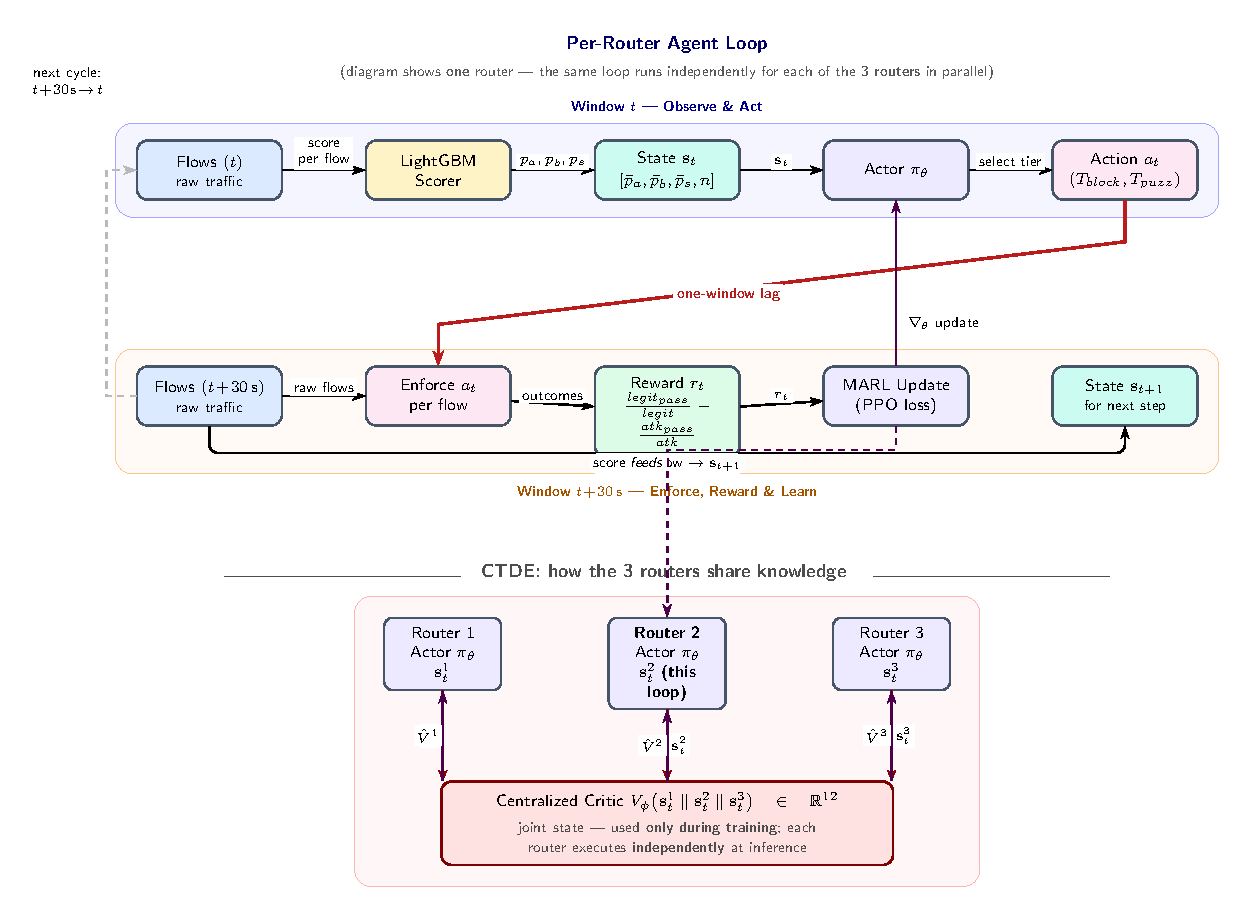
\includegraphics[width=0.92\textwidth]{fig_env_loop.pdf}
\caption{Per-router agent loop in CoopIDS. \textbf{Window $t$ (top, blue):} flows are scored by LightGBM, aggregated into a 4-dim state $\mathbf{s}_t$, and fed to the MAPPO actor which selects a tiered action $a_t = (T_\text{block}, T_\text{puzz})$. \textbf{Window $t\!+\!30\,\mathrm{s}$ (bottom, orange):} the selected profile is enforced per-flow on the new window's traffic; outcomes determine the reward $r_t$, which drives the PPO update. The red arrow indicates the one-window lag between action selection and enforcement; the dashed grey arrow represents the cycle reset ($t\!+\!30\,\mathrm{s} \to t$). \textbf{CTDE panel (bottom):} during training only, the centralized critic $V_\phi(\mathbf{s}^1_t \| \mathbf{s}^2_t \| \mathbf{s}^3_t) \in \mathbb{R}^{12}$ aggregates the joint state of all three routers to produce per-agent value estimates $\hat{V}^i$. At inference, each router executes its actor independently.}
\label{fig:envloop}
\end{figure*}


%% ═══════════════════════════════════════════════════════════════════
\section{Experimental Results}
\label{sec:results}

We evaluate CoopIDS through a comprehensive 40-stage ablation study (S1--S40), systematically isolating the contributions of the risk sensor, action design, cooperation mechanism, reward structure, and agent scaling.

\subsection{Experimental Setup}

All experiments use the hyperparameters listed in Table~\ref{tab:hyperparams}. These were fixed across the entire tiered architecture phase (S26--S40) to ensure comparability. Actor and critic learning rates were chosen based on standard PPO guidance: a higher critic learning rate accelerates value function convergence, while a conservative actor learning rate prevents policy collapse. The GAE parameters ($\gamma = 0.99$, $\lambda = 0.95$) favour long-horizon credit assignment, appropriate for our 968-step episodes where early actions influence late-episode attack blocking performance.

\begin{table}[t]
\centering
\small
\caption{Hyperparameters (fixed across all tiered experiments S26--S40).}
\label{tab:hyperparams}
\begin{tabular}{lrl}
\toprule
Parameter & Value & Description \\
\midrule
$N$ (agents) & 3 & Edge routers \\
State dim & 4 & $[\bar{p}_\text{atk}, \bar{p}_\text{ben}, \bar{p}_\text{sus}, \bar{n}]$ \\
Joint dim & 12 & Concatenated states (critic) \\
Action dim & 6 & Tiered profiles \\
Hidden dim & 128 & Actor \& critic hidden layers \\
$\gamma$ & 0.99 & Discount factor \\
$\lambda_\text{GAE}$ & 0.95 & GAE trace decay \\
$\epsilon_\text{clip}$ & 0.2 & PPO clipping threshold \\
$\alpha_\text{actor}$ & $3 \times 10^{-4}$ & Actor learning rate \\
$\alpha_\text{critic}$ & $1 \times 10^{-3}$ & Critic learning rate \\
Entropy coeff. & 0.01 & Exploration bonus \\
Update freq. & 10 ep. & PPO update interval \\
PPO epochs & 4 & Epochs per update batch \\
Mini-batch size & 64 & PPO mini-batch \\
Episodes & 500 & Total training episodes \\
Window size & 30\,s & Flow aggregation window \\
\bottomrule
\end{tabular}
\end{table}

\subsection{Evaluation Protocol}

All models are trained exclusively on Monday data and evaluated on both Monday (seen attacks) and Tuesday (unseen attacks) without any weight modification. Evaluation replays the complete day's traffic through the trained agents using greedy action selection (no exploration). Evaluation metrics are:

\begin{itemize}
    \item \textbf{True Positive Rate (TPR):} fraction of attack flows correctly stopped.
    \item \textbf{False Positive Rate (FPR):} fraction of benign flows incorrectly stopped.
    \item \textbf{Precision:} fraction of blocked flows that are true attacks, $\text{Precision} = \frac{\text{TPR} \cdot n_\text{atk}}{\text{TPR} \cdot n_\text{atk} + \text{FPR} \cdot n_\text{ben}}$.
    \item \textbf{F1 Score:} harmonic mean of Precision and TPR, $F_1 = \frac{2 \cdot \text{Precision} \cdot \text{TPR}}{\text{Precision} + \text{TPR}}$. Used as the primary metric given the class imbalance (9.6\% attack flows on Tuesday).
    \item \textbf{Legitimate Ratio:} fraction of benign flows that pass through ($1 - \text{FPR}$).
\end{itemize}

Importantly, TPR is measured at the \emph{flow level}, not the window level: every individual flow is classified as blocked or passed based on the agent's selected tiered profile and the flow's $p_\text{risk}$ score. This provides a more accurate measure than window-level detection, since a single window may contain both benign and attack flows that should be treated differently.

\subsection{Baseline Comparison}

Several observations emerge from the early ablation stages. IQL (S6) achieves only 89.6\% Monday TPR with 15.2\% FPR---the non-stationarity of independent Q-learning in a multi-agent environment prevents effective coordination. IPPO (S7) and MAPPO (S8--S9) both reach $\sim$95\% Monday TPR with a 10-action throttle space, but generalisation to Tuesday is limited and the action space lacks the structured risk-threshold coupling that characterises the tiered design. These results motivate the transition to tiered action profiles (Section~\ref{sec:tiers}), where each discrete action encodes a coherent defensive posture calibrated from the Monday $p_\text{risk}$ distribution.

\subsection{Tiered Architecture Results}

Table~\ref{tab:tiered} presents the results of the tiered action profile architecture.

\begin{table*}[t]
\centering
\small
\caption{Full results on unseen Tuesday attacks (zero-shot generalisation). All models trained on Monday only, evaluated on Tuesday without retraining. Precision, F1 derived from TPR, FPR, and Tuesday class distribution (9.6\% attack, 58.5\% benign, $n=85{,}479$). Legit $= 1 - \text{FPR}$. S30 uses a combined Monday+Tuesday LightGBM sensor; all others use Monday-only. LightGBM only (no RL) uses argmax class prediction directly.}
\label{tab:tiered}
\begin{tabular}{llccccc}
\toprule
Model & Stage & TPR$\uparrow$ & FPR$\downarrow$ & Precision$\uparrow$ & F1$\uparrow$ & Legit$\uparrow$ \\
\midrule
\multicolumn{7}{l}{\textit{Baseline (no RL policy)}} \\
\midrule
LightGBM only (no RL)             & ---  & 37.02\% & 0.42\% & 93.58\% & 53.05\% & 99.58\% \\
\midrule
\multicolumn{7}{l}{\textit{Tiered action profiles ($p_\text{risk}$ routing, 6 profiles)}} \\
\midrule
MAPPO tiered (local)              & S27  & 85.78\% & 6.01\% & 70.08\% & 77.14\% & 93.99\% \\
IPPO tiered (no CTDE)             & S29  & 88.38\% & 7.71\% & 65.29\% & 75.10\% & 92.29\% \\
MAPPO + retrained LightGBM        & S30  & \textbf{94.68\%} & \textbf{1.17\%} & \textbf{93.00\%} & \textbf{93.83\%} & \textbf{98.83\%} \\
MAPPO + MLP encoder               & S39  & 83.96\% & 5.74\% & 70.59\% & 76.70\% & 94.26\% \\
MAPPO + global reward             & S40  & 87.88\% & 7.20\% & 66.70\% & 75.84\% & 92.80\% \\
\bottomrule
\end{tabular}
\end{table*}

Figure~\ref{fig:results} visualises the Monday--Tuesday TPR gap across all model variants.

\begin{figure*}[t]
\centering
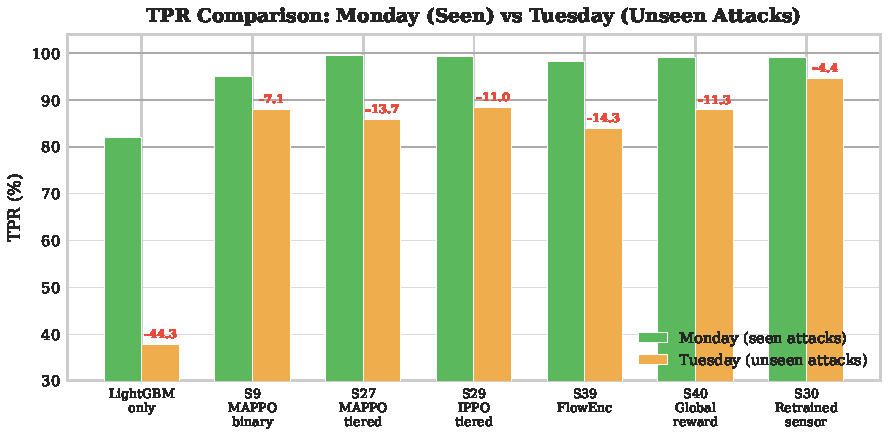
\includegraphics[width=\textwidth]{fig_results_comparison.pdf}
\caption{TPR comparison across all model variants. Green bars: Monday (seen attacks). Orange bars: Tuesday (unseen attacks). Red annotations show the generalisation drop. S30 (retrained sensor) achieves the smallest drop ($-4.4$pp), demonstrating that sensor quality---not the MARL policy---is the bottleneck.}
\label{fig:results}
\end{figure*}

The tiered architecture dramatically outperforms the baselines. S27 achieves 99.52\% Monday TPR (vs.\ 95\% for the best baseline) while reducing FPR from 4.95\% to 2.91\%. On the harder Tuesday zero-shot test, the RL policy raises F1 from 53.05\% (LightGBM alone, no RL) to 77.14\%---a 24pp gain. S27 further achieves 85.78\% TPR on 5 completely unseen attack types with the same trained weights, confirming zero-shot generalisation.

When only the LightGBM sensor is retrained on combined Monday+Tuesday data (S30), the same MARL policy achieves 94.68\% TPR with 1.17\% FPR and F1 = 93.83\%---a 16.7pp F1 gain over S27 without any RL retraining. This isolates the Sensor as the generalisation bottleneck: the \emph{learned policy generalises; the risk sensor does not}.

S39, which replaces Lightgbm with a jointly-trained MLP encoder, actually decreases Tuesday TPR to 83.96\%---1.8pp below the frozen LightGBM baseline---confirming that gradient-boosted ensemble feature engineering provides stronger generalisation than joint neural training.

\subsection{Cooperation Ablation: MAPPO vs IPPO}

Comparing S27 (MAPPO) and S29 (IPPO) isolates the contribution of the centralised critic. On Monday, the difference is negligible ($<$0.2pp). On Tuesday, IPPO achieves 2.6pp higher TPR (88.38\% vs. 85.78\%), but at the cost of 1.7pp higher FPR (7.71\% vs. 6.01\%). When both are taken into account via F1, MAPPO holds a slight edge: 77.14\% vs. 75.10\%---meaning IPPO's extra attack detections are outweighed by its additional false alarms. The CTDE mechanism provides no clear advantage at 3 routers in terms of raw TPR, but it does produce a more balanced Precision--recall trade-off.

However, scaling to 6 routers reveals the true value of cooperation. Table~\ref{tab:scaling} shows that MAPPO degrades gracefully ($-1.0$pp Tuesday TPR) while IPPO collapses ($-30.3$pp), as independent agents fail at credit assignment when the coordination requirements increase.

\begin{table}[t]
\centering
\small
\caption{Scaling from 3 to 6 routers: MAPPO vs IPPO.}
\label{tab:scaling}
\begin{tabular}{lcccc}
\toprule
\multirow{2}{*}{Model} & \multicolumn{2}{c}{3 Routers} & \multicolumn{2}{c}{6 Routers} \\
\cmidrule(lr){2-3} \cmidrule(lr){4-5}
 & Mon TPR & Tue TPR & Mon TPR & Tue TPR \\
\midrule
MAPPO (CTDE)    & 99.52\% & 85.78\% & 98.98\% & 84.76\% \\
IPPO (no CTDE)  & 99.35\% & 88.38\% & 97.47\% & 58.13\% \\
\midrule
$\Delta$ (3$\to$6) & --- & --- & $-$0.54pp & $-$1.0pp / $-$30.3pp \\
\bottomrule
\end{tabular}
\end{table}

\subsection{End-to-End Learning: FlowEncoder (S39)}

S39 replaces the frozen LightGBM risk scorer with a jointly-trained neural encoder (FlowEncoder), a 3-layer MLP:
$$42 \xrightarrow{\text{Linear}} 64 \xrightarrow{\text{BN+ReLU}} 32 \xrightarrow{\text{BN+ReLU}} \begin{cases} 3\text{-dim embedding} \\ 1\text{-dim risk (sigmoid)}\end{cases}$$

The encoder is warm-started with 20 epochs of supervised BCE training (target: 1.0 for attack/suspicious, 0.0 for benign), then co-trained with the MAPPO policy---the encoder receives a supervised update every 10 episodes alongside the PPO update. Input features are standardised (zero-mean, unit-variance) since neural networks, unlike gradient-boosted trees, require normalised inputs.

Despite joint training, S39 achieves only 83.96\% Tuesday TPR---1.8pp \emph{below} the frozen LightGBM baseline (S27). Two factors explain this: (1) gradient-boosted trees are inherently better at tabular data than shallow MLPs~\cite{grinsztajn2022tree}, and (2) joint training creates competing gradients where the encoder may optimise for features useful to the current policy rather than maintaining a broadly discriminative risk score. This negative result reinforces the sensor bottleneck finding: improving generalisation requires better risk scoring, and naive end-to-end training may be counterproductive.

\subsection{Reward Structure: Local vs Global}

Comparing S27 (local reward, each agent scored on its own flows) with S40 (global reward, single shared reward across all agents), we find that S40 achieves marginally higher Tuesday TPR (87.88\% vs. 85.78\%), but S27 holds a better F1 (77.14\% vs. 75.84\%) due to lower FPR. The difference is small in both directions, suggesting that at 3 agents, the reward structure is not a critical design choice---a useful negative result for practitioners.

\subsection{Ablation Study: S1--S40 Progression}

Our 40-stage ablation study evolved through four phases:

\textbf{Phase 1 (S1--S5):} Single-agent experiments establishing that LightGBM risk scoring is essential (S3 vs S1: +25pp TPR) and that per-flow decisions outperform blind throttling.

\textbf{Phase 2 (S6--S9):} Multi-agent baselines demonstrating that IQL fails due to non-stationarity, while MAPPO and IPPO achieve comparable performance with 10-action throttle spaces but lack the structured risk-threshold coupling needed for effective generalisation.

\textbf{Phase 3 (S10--S22):} Architecture variations exploring state augmentation, reward shaping, and curriculum learning---all providing marginal improvements, confirming that action space design is the key lever.

\textbf{Phase 4 (S26--S40):} Tiered action profiles with Monday-calibrated thresholds, enabling systematic ablation of sensor quality (S30), encoder architecture (S39), reward structure (S40), and agent scaling (S31, S37).

\subsection{Training Efficiency}

Training S27 requires 500 episodes with PPO updates every 10 episodes. Each episode replays the full Monday data ($\sim$968 windows), taking approximately 2.7 seconds for forward passes and 7.5 seconds including PPO updates. Total training time is $\approx$23 minutes on a single CPU---making the approach practical for rapid experimentation.


%% ═══════════════════════════════════════════════════════════════════
\section{Discussion}
\label{sec:discussion}



\subsection{The Sensor Bottleneck}

Our most significant finding is that policy generalisation is not the bottleneck---sensor generalisation is. The MARL policy learned on S27 (with Monday-only LightGBM) achieves 85.78\% Tuesday TPR. The \emph{exact same policy} with a retrained sensor (S30) achieves 94.68\%. This 8.9pp improvement requires zero RL retraining, demonstrating that investing in better risk scoring (e.g., online adaptive models, continual learning) directly translates to better defence without modifying the cooperative policy.

\subsection{CTDE at Scale}

The value of CTDE is not apparent at 3 routers, where IPPO matches or exceeds MAPPO on raw TPR. However, at 6 routers, IPPO's Tuesday TPR drops by 30.3pp while MAPPO's drops by only 1.0pp. The centralised critic provides implicit coordination: it learns that when one router tightens its policy, others can maintain looser profiles, distributing the filtering burden. Without this signal, independent agents over-filter or under-filter, with the penalty growing combinatorially with agent count.



\subsection{Training Dynamics}

Figure~\ref{fig:training} shows the S27 reward curve. The reward shows rapid initial improvement from $\sim$780 (episodes 1--9, before any PPO update) to $\sim$900 after the first update at episode 10. Convergence to the final reward of $\sim$922 occurs by episode $\sim$200, with the remaining episodes providing incremental refinement.

\begin{figure}[t]
\centering
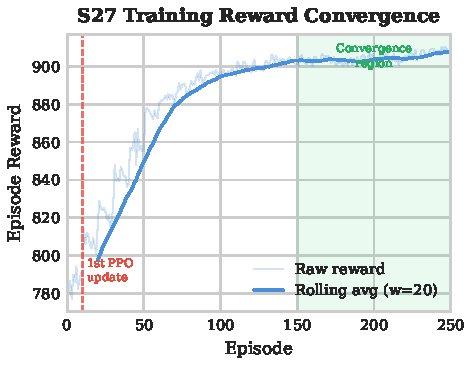
\includegraphics[width=\columnwidth]{fig_training_curve.pdf}
\caption{S27 training reward over 250 episodes. The vertical dashed line marks the first PPO update (episode 10). The shaded region indicates convergence ($>$200 episodes).}
\label{fig:training}
\end{figure} The early convergence suggests that the tiered action space, combined with strong LightGBM state signals, provides a well-shaped learning landscape. Forward passes take $\sim$2.7 seconds per episode, while PPO update steps add $\sim$4.8 seconds, yielding total training time of approximately 23 minutes on a single CPU.

The entropy coefficient ($0.01$) provides sufficient exploration early in training while naturally decaying as the policy becomes more confident.

\subsection{Limitations}

Several limitations merit discussion. First, our Environment replays recorded traffic rather than simulating adaptive attackers. An adversary who learns to mimic benign flow features could degrade the risk scorer's accuracy, though this attack vector targets the sensor (already identified as the bottleneck), not the MARL policy. Second, the 3-router topology, while sufficient to demonstrate cooperation, is smaller than production ISP deployments. Our scaling experiments (3 vs 6 routers) provide initial evidence that MAPPO scales, but validation at 9--12 routers is needed. Finally, the LightGBM risk scorer is frozen during MARL training, precluding joint adaptation of the sensor and policy. Our S39 experiment with a jointly-trained MLP encoder actually performed worse, suggesting that naive joint training may be counterproductive.


%% ═══════════════════════════════════════════════════════════════════
\section{Conclusion}
\label{sec:conclusion}

We presented CoopIDS, a cooperative MARL framework for DDoS mitigation at ISP edge routers. By combining per-flow LightGBM risk scoring with tiered action profiles and MAPPO with CTDE, CoopIDS generalises zero-shot to 5 unseen attack types with F1 = 93.83\% (using a retrained sensor) or F1 = 77.14\% (with the original sensor)---compared to F1 = 53.05\% for the LightGBM classifier alone, while preserving 98.83\% of legitimate traffic.

Our 40-stage ablation study yields three principal findings: (1) tiered action profiles force agents to learn effective blocking policies, producing a 4.5pp TPR improvement over binary action baselines; (2) the learned policy generalises to unseen attacks, but the risk sensor does not---retraining only the sensor (no RL retraining) recovers 8.9pp on unseen attacks; and (3) CTDE provides critical scaling benefits, with MAPPO degrading only 1.0pp at 6 routers while IPPO collapses by 30.3pp.

Several promising directions emerge from our findings:

\textbf{Online adaptive risk scoring.} The most impactful improvement would replace the frozen LightGBM with an online adaptive model (e.g., Adaptive Random Forest or continual-learning neural network) that updates its feature representations as new attack patterns emerge.

\textbf{Testbed validation.} CoopIDS currently operates on recorded traffic replay, where challenge outcomes are modelled via fixed pass rates. Validating the tiered filtering mechanism on a live network testbed would confirm whether these assumptions hold in practice and provide more realistic reward signals during training.

\textbf{Larger topologies.} Scaling to 9--12 routers with hierarchical coordination mechanisms (e.g., HAPPO~\cite{kuba2022trust} or GNN-based communication) would test whether CTDE benefits continue to scale or whether communication becomes necessary.

\textbf{Adversarial evaluation.} An adaptive attacker that learns to mimic benign flow features would test the robustness of both the risk scorer and the MARL policy under worst-case conditions.


%% ═══════════════════════════════════════════════════════════════════
\bibliographystyle{ACM-Reference-Format}

\begin{thebibliography}{10}

\bibitem{bccc2024}
A.~Hayati, K.~Shahbar, and A.~B.~Osman.
\newblock {BCCC-cPacket-Cloud-DDoS-2024}: A real-world cloud DDoS dataset.
\newblock In \emph{Proc. Canadian Institute for Cybersecurity}, 2024.

\bibitem{breiman2001random}
L.~Breiman.
\newblock Random forests.
\newblock \emph{Machine Learning}, 45(1):5--32, 2001.

\bibitem{han2021marl}
J.~Han, et al.
\newblock Multi-agent reinforcement learning for network defence: A survey.
\newblock \emph{IEEE Communications Surveys \& Tutorials}, 23(4):2227--2259, 2021.

\bibitem{ke2017lightgbm}
G.~Ke, Q.~Meng, T.~Finley, et al.
\newblock {LightGBM}: A highly efficient gradient boosting decision tree.
\newblock In \emph{Advances in Neural Information Processing Systems (NeurIPS)}, pp.~3146--3154, 2017.

\bibitem{lowe2017multi}
R.~Lowe, Y.~Wu, A.~Tamar, et al.
\newblock Multi-agent actor-critic for mixed cooperative-competitive environments.
\newblock In \emph{Advances in Neural Information Processing Systems (NeurIPS)}, pp.~6379--6390, 2017.

\bibitem{malialis2015distributed}
K.~Malialis and D.~Kudenko.
\newblock Distributed response to network intrusions using multiagent reinforcement learning.
\newblock \emph{Engineering Applications of Artificial Intelligence}, 41:270--284, 2015.

\bibitem{mirkovic2004taxonomy}
J.~Mirkovic and P.~Reiher.
\newblock A taxonomy of {DDoS} attack and {DDoS} defense mechanisms.
\newblock \emph{ACM SIGCOMM Computer Communication Review}, 34(2):39--53, 2004.

\bibitem{roesch1999snort}
M.~Roesch.
\newblock Snort: Lightweight intrusion detection for networks.
\newblock In \emph{Proc. USENIX LISA}, pp.~229--238, 1999.

\bibitem{schulman2015high}
J.~Schulman, P.~Moritz, S.~Levine, M.~Jordan, and P.~Abbeel.
\newblock High-dimensional continuous control using generalized advantage estimation.
\newblock In \emph{Proc. ICLR}, 2016.

\bibitem{schulman2017proximal}
J.~Schulman, F.~Wolski, P.~Dhariwal, A.~Radford, and O.~Klimov.
\newblock Proximal policy optimization algorithms.
\newblock \emph{arXiv preprint arXiv:1707.06347}, 2017.

\bibitem{yu2022surprising}
C.~Yu, A.~Velu, E.~Vinitsky, et al.
\newblock The surprising effectiveness of {PPO} in cooperative multi-agent games.
\newblock In \emph{Advances in Neural Information Processing Systems (NeurIPS)}, 2022.

\bibitem{wang2003detecting}
X.~Wang and M.~K.~Reiter.
\newblock Defending against denial-of-service attacks with puzzle auctions.
\newblock In \emph{Proc. IEEE Symposium on Security and Privacy}, pp.~78--92, 2003.

\bibitem{kuba2022trust}
J.~Kuba, R.~Chen, M.~Wen, et al.
\newblock Trust region policy optimisation in multi-agent reinforcement learning.
\newblock In \emph{Proc. ICLR}, 2022.

\bibitem{grinsztajn2022tree}
L.~Grinsztajn, E.~Oyallon, and G.~Varoquaux.
\newblock Why do tree-based models still outperform deep learning on typical tabular data?
\newblock In \emph{Advances in Neural Information Processing Systems (NeurIPS)}, 2022.

\bibitem{mirsky2018kitsune}
Y.~Mirsky, T.~Doitshman, Y.~Elovici, and A.~Shabtai.
\newblock Kitsune: An ensemble of autoencoders for online network intrusion detection.
\newblock In \emph{Proc. NDSS Symposium}, 2018.

\bibitem{de2020independent}
C.~de~Witt, T.~Gupta, D.~Makoviichuk, et al.
\newblock Is independent learning all you need in the {StarCraft} multi-agent challenge?
\newblock \emph{arXiv preprint arXiv:2011.09533}, 2020.

\end{thebibliography}

\end{document}
